% !TEX encoding = UTF-8
%Koma article
\documentclass[fontsize=12pt,paper=letter,twoside]{scrartcl}
\usepackage{float}
\usepackage{listings}
\usepackage{makecell}

%Standard Pre-amble
\usepackage[top=4cm,bottom=4cm,left=3cm,right=3cm,asymmetric]{geometry}
%\geometry{landscape}                % Activate for for rotated page geometry
%\usepackage[parfill]{parskip}    % Begin paragraphs with an empty line rather than an indent
\usepackage[table,xcdraw]{xcolor}
\usepackage{graphicx}

\usepackage{amsmath}
\usepackage{amssymb}
\usepackage{epstopdf}
\DeclareGraphicsRule{.tif}{png}{.png}{`convert #1 `dirname #1`/`basename #1 .tif`.png}
% Listings needs package courier
\usepackage{listings} % Needs 
\usepackage{courier}

\usepackage[framemethod=TikZ]{mdframed}
\usepackage{url}

\usepackage{sty/bsymb} %% Event-B symbols
\usepackage{sty/eventB} %% REQ and ENV
\usepackage{sty/calculation}

%Maths
\usepackage{amssymb,amsmath}
\def\Fl{\mathbb{F}}
\def\Rl{\mathbb{R}}
\def\Nl{\mathbb{N}}
\def\Bl{\mathbb{B}}
\def\St{\mathbb{S}}
\newcommand{\ovr}{\upharpoonright}
\newcommand{\var}[1]{\textit{#1}}
%Useful definitions
\newcommand{\mv}[1]{\textit{m\_#1}}
\newcommand{\cv}[1]{\textit{c\_#1}}
\newcommand{\degree}[1]{^{\circ}\mathrm{#1}}
%\newcommand{\comment}[1]{{\footnotesize \quad\texttt{--}\textrm{#1}}}
\newcommand{\im}[1]{i\texttt{-\!#1}}

\usepackage[headsepline]{scrpage2}
\pagestyle{scrheadings}
\ihead[]{\small EECS4312 Report1}
\ohead[]{\small \thepage}
\cfoot[]{}
\ofoot[]{}


%%%%PVS environment%%%%%%%%%%%%%%%%%%%
\lstnewenvironment{pvs}[1][]
    {\lstset{#1,captionpos=b,language=pvs,
    mathescape=true,
    basicstyle=\small\ttfamily,
    numbers=none,
    frame=single,
    % numberstyle=\tiny\color{gray},
    % backgroundcolor=\color{lightgray},
    firstnumber=auto
    }}
    {}
 %%%%%%%%%%%%%%%%%%%%%%%%%%%%%%%%
 
%%%%Verbatim environment%%%%%%%%%%%%%%%%%%%
\lstnewenvironment{code}[1][]
    {\lstset{#1,captionpos=b,
    mathescape=true,
    basicstyle=\small\ttfamily,
    numbers=none,
    frame=single,
    % numberstyle=\tiny\color{gray},
    % backgroundcolor=\color{lightgray},
    firstnumber=auto
    }}
    {}

% \newenvironment{boxed}[1]
%    {\begin{center}
%    #1\\[1ex]
%    \begin{tabular}{|p{0.9\textwidth}|}
%    \hline\\
%    }
%    { 
%    \\\\\hline
%    \end{tabular} 
%    \end{center}
%    }
 %%%%%%%%%%%%%%%%%%%%%%%%%%%%%%%%
 
 %Text in a box
\newenvironment{textbox}
    {\begin{center}
    \begin{tabular}{|p{0.9\textwidth}|}
    \hline\\
    }
    { 
    \\\\\hline
    \end{tabular} 
    \end{center}
    }

\usepackage{hyperref}

%Highlight \hl{}
\usepackage{soul}

\usepackage{enumitem}
\newlist{mylist}{itemize}{1}
\setlist[mylist]{label=\textbullet,leftmargin=1cm,nosep}

\usepackage{multirow}

% Reduce space between figure and caption
%\usepackage{caption}
%\captionsetup[table]{font=small,skip=0pt}     %% Adjust here
%or equivalently 
\usepackage[font=small,skip=4pt]{caption}
%Useful definitions
%\newcommand{\mv}[1]{\textit{m\_#1}}
%\newcommand{\cv}[1]{\textit{c\_#1}}
%\newcommand{\degree}[1]{^{\circ}\mathrm{#1}}
%\newcommand{\comment}[1]{{\footnotesize \quad\texttt{--}\textrm{#1}}}


%For Code Stylings
\usepackage{listings}
\usepackage{color}

\definecolor{dkgreen}{rgb}{0,0.6,0}
\definecolor{gray}{rgb}{0.5,0.5,0.5}
\definecolor{mauve}{rgb}{0.58,0,0.82}

\lstset{frame=tb,
  language=Java,
  aboveskip=3mm,
  belowskip=3mm,
  showstringspaces=false,
  columns=flexible,
  basicstyle={\small\ttfamily},
  numbers=none,
  numberstyle=\tiny\color{gray},
  keywordstyle=\color{blue},
  commentstyle=\color{dkgreen},
  stringstyle=\color{mauve},
  breaklines=true,
  breakatwhitespace=true,
  tabsize=3
}

% Set the header
\ihead[]{\small EECS4313 Assignment-3}


%%%%%%%%%%%%Enter your names here%%%%%%%%
\author{Student Name | Student Number | EECS Account
\and \textbf{Edward Vaisman | 212849857 | eddyv}
\and \textbf{Robin Bandzar | 212200531 | cse23028}
\and \textbf{Kirusanth Thiruchelvam | 212918298 | kirusant}
\and \textbf{Sadman Sakib Hasan | 212497509 | cse23152}
}
%%%%%%%%%%%%%%%%%%%%%%%%%%%%%%%%

\date{\today} % Display a given date or no date

\begin{document}
\title{EECS 4313 Assignment 3 \\Data Flow Testing, Slice-Based Testing and Mutation Testing}
\maketitle

\newpage

%%%%%%%%%%%%%%%%%%%%%%%%%%%%%%%
\tableofcontents


\newpage


\section{BORG Calendar}

\subsection{Mutation Testing}
Mutation tests were run using the previous unit test suite that we created for assignment 2. The program used to run the Mutation tests was \emph{Eclispe} with the \emph{Pitclipse} plugin. The three methods that we tested are listed with their results in the following subsections. 

\subsubsection{minuteString}


\begin{figure}[H]
\begin{center}
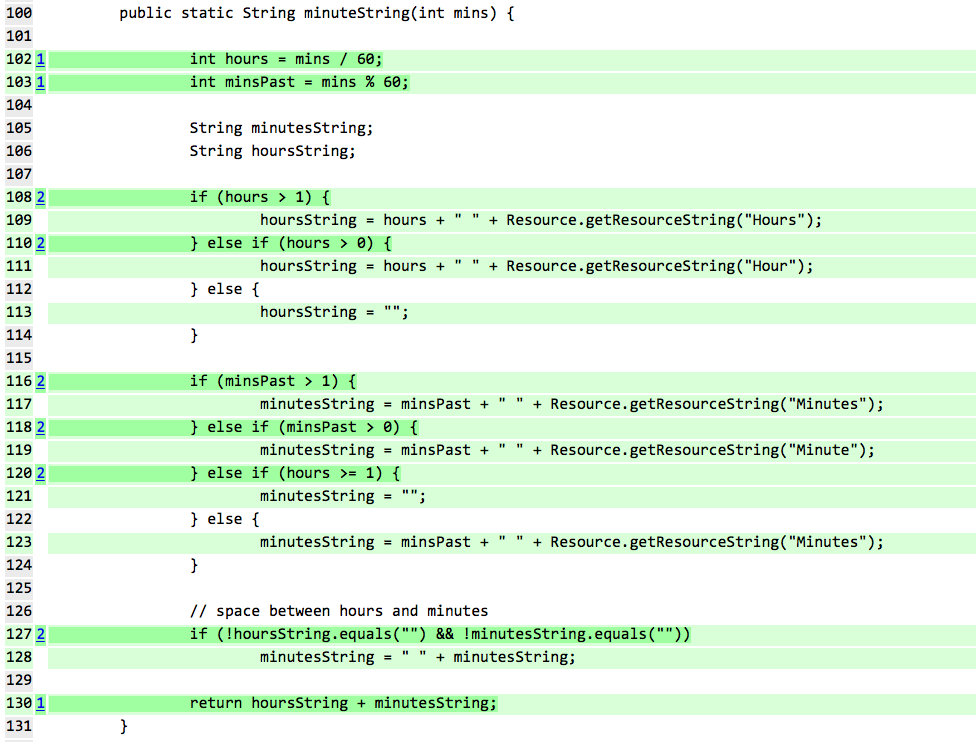
\includegraphics[width=.99\textwidth]{images/MutationTesting/minuteStringCode.png}
\end{center}
\caption{Code for the minuteString method}
\label{fig:minuteStringCode}
\end{figure}

\begin{figure}[H]
\begin{center}
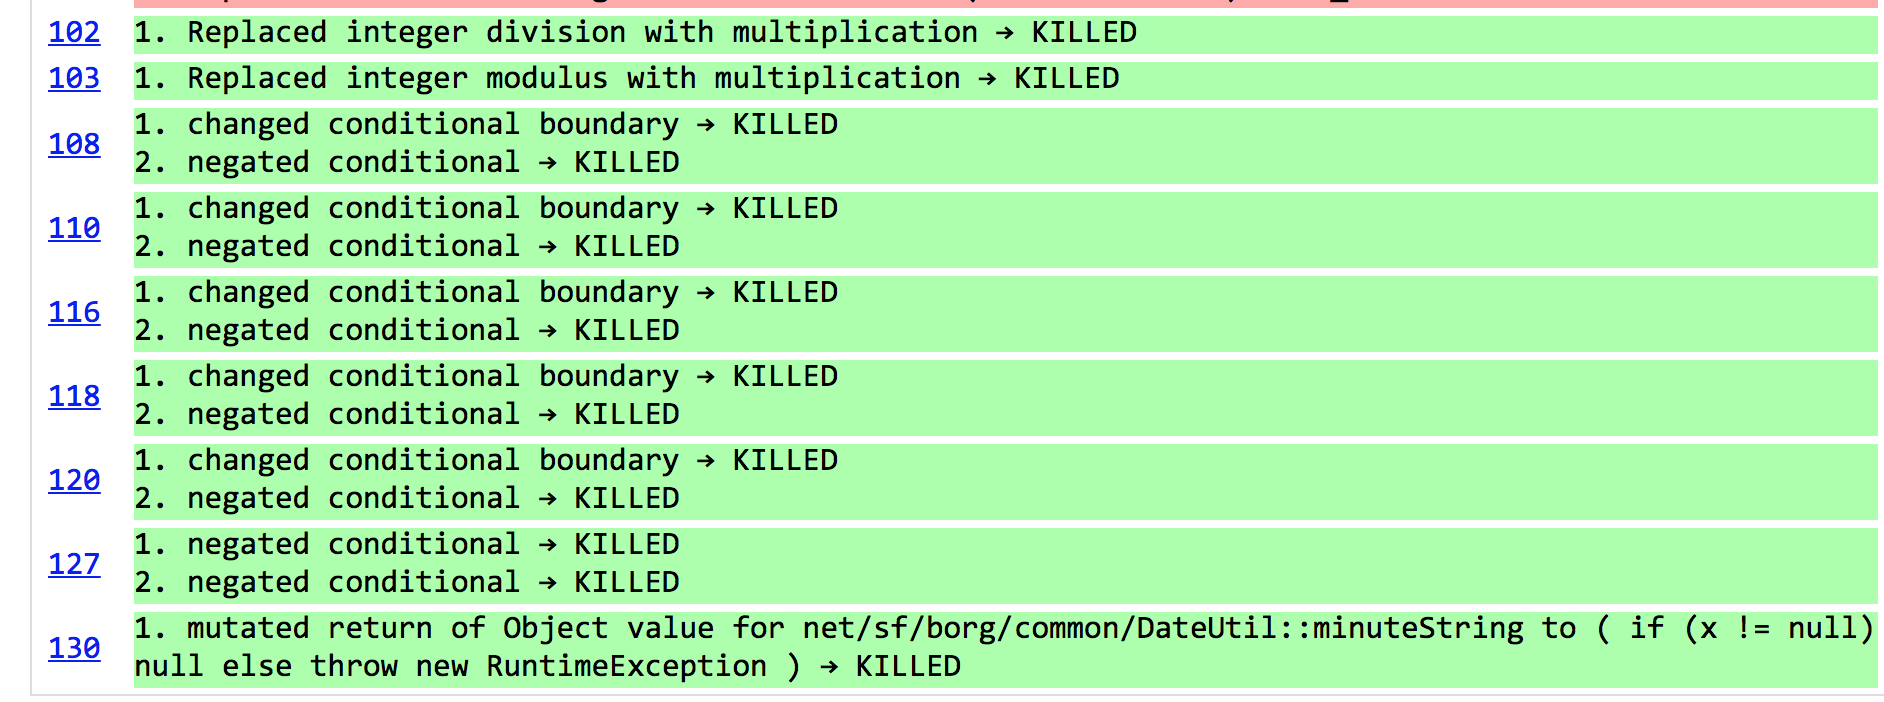
\includegraphics[width=.99\textwidth]{images/MutationTesting/minuteStringMutant.png}
\end{center}
\caption{Mutations for the minuteString method}
\label{fig:minuteStringMutant}
\end{figure}

As one can see in Figures \ref{fig:minuteStringCode} and \ref{fig:minuteStringMutant} that the previous tests effectively kill all the mutants so no further changes are needed.

\subsubsection{isAfter}
\begin{figure}[H]
\begin{center}
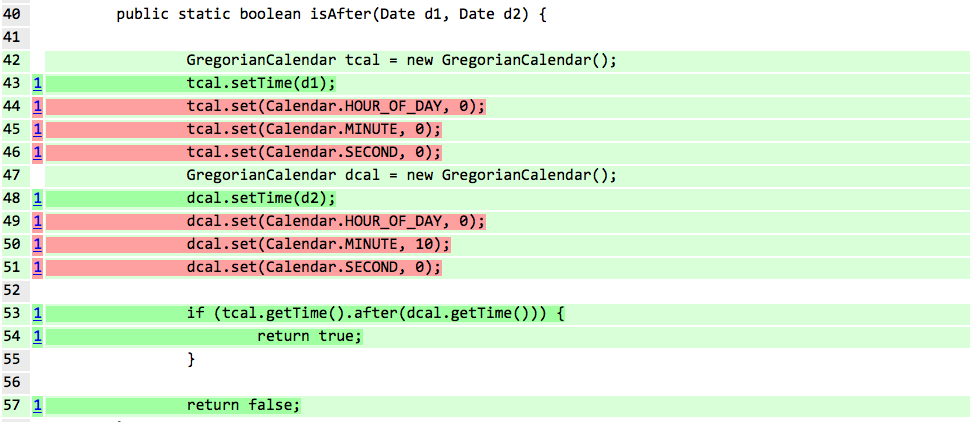
\includegraphics[width=.99\textwidth]{images/MutationTesting/isAfterCode.png}
\end{center}
\caption{Code for the isAfter method}
\label{fig:isAfterCode}
\end{figure}

\begin{figure}[H]
\begin{center}
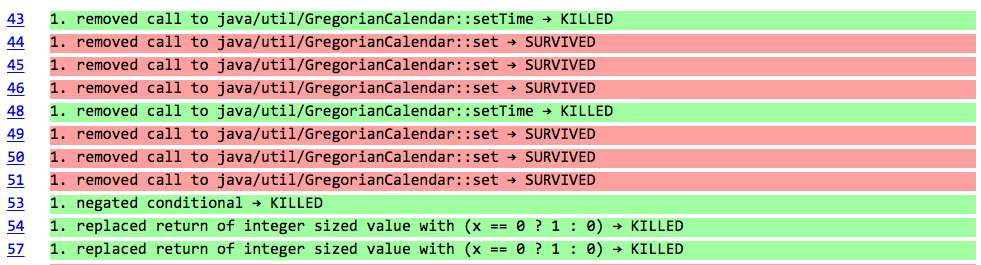
\includegraphics[width=.99\textwidth]{images/MutationTesting/isAfterMutant.png}
\end{center}
\caption{Mutations for the isAfter method on OSX}
\label{fig:isAfterMutant}
\end{figure}
\setlength\intextsep{0pt}
The two Figures above show that the previous tests have mutants which survived.


\subsubsection{sendMsg}
\begin{figure}[H]
\begin{center}
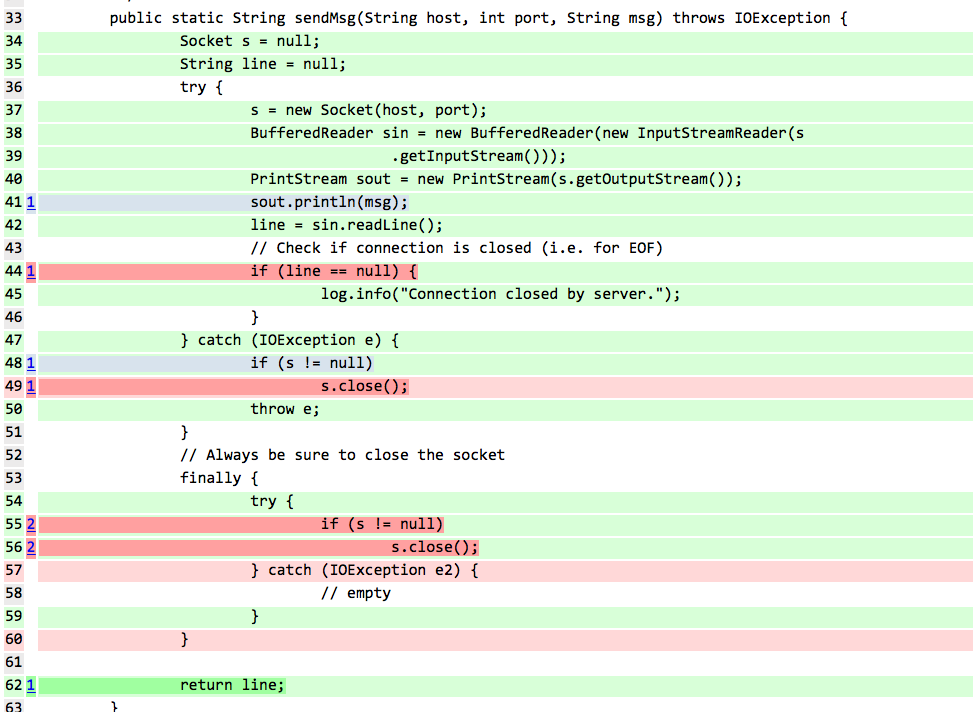
\includegraphics[width=.99\textwidth]{images/MutationTesting/sendMsgCode.png}
\end{center}
\caption{Code for the sendMsg method}
\label{fig:sendMsgCode}
\end{figure}

\begin{figure}[H]
\begin{center}
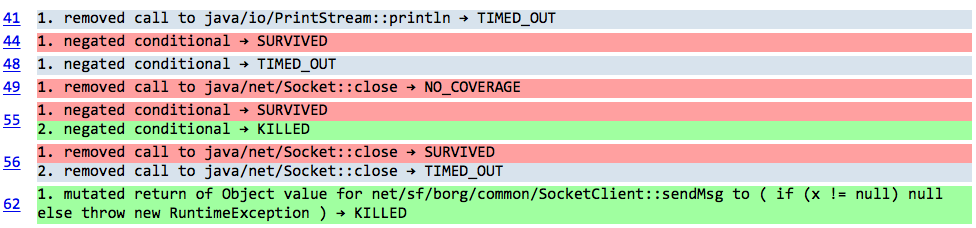
\includegraphics[width=.99\textwidth]{images/MutationTesting/sendMsgMutant.png}
\end{center}
\caption{Mutations for the sendMsg method on OSX}
\label{fig:sendMsgMutant}
\end{figure}

The results show that not all mutants have been killed.

\begin{itemize}
\item The data flow analysis you performed and the calculation of the coverage metrics. You must
show which test cases are responsible for which dc-paths.
\item A description of the test cases you added to improve coverage. If your coverage was already high,
discuss how your testing was able to achieve this.
\item The slices that you identified and the percentage of slices that your testing covers. You must
show which test cases are responsible for which slices.
\item A description of the test cases you added to improve slice coverage. If your coverage was
already high, discuss how your testing was able to achieve this.
\item Evaluate the effectiveness of your test cases using mutation testing. Discuss and address any
issues if you have found in your written report.
\item Attaching bug reports if bugs are discovered using your testing methods. You should use the
same bug report format as in Assignment 1. Do not file these bug reports to the project’s bug
report system.
\item An appendix with the specification of the methods you are testing
\end{itemize}

\section{JPetStore}

\begin{itemize}
\item The test scenarios that you have created;
\item The request rates and the duration of the load tests;
\item The analysis of your load tests and the description of any problems that you have found (if there
are any).
\end{itemize}

\end{document}
